\section{Seamless Development} \label{chapter3:objectives}

\begin{figure}[h!] \label{fig:state-of-the-art-proposition}
\begin{center}
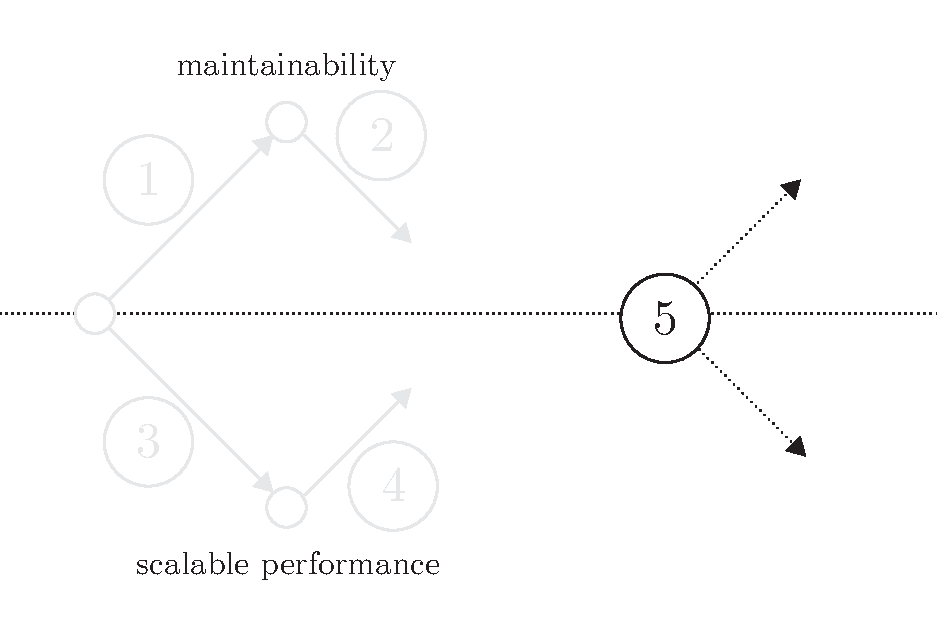
\includegraphics[width=0.6\textwidth]{../ressources/state-of-the-art-5.pdf}
\end{center}
\end{figure}



The section \ref{chapter3:software-maintainability} shows that the modular organization enabled by functional programming is the best way to improve maintainability.
But it requires the use of a global memory store which conflicts with performance.
Compilation is a solution to reduce this conflict, but is not yet satisfactory enough for high performance scalability.
On the other hand, the section \ref{chapter3:software-performance} shows that to attain performance scalability, an application needs to multiply the exclusive accesses to its state.
That implies to follow a distributed organization of its state to provide isolation and immutability, which negatively impacts modularity, hence maintainability.
Some works provide a uniform memory access to improve maintainability, despite the distributed execution.

The evolution of the economical constraints of a web application requires to repeatedly switch between maintainability and performance scalability.
The incompatibility between the two organizations implies technological ruptures at each switch.
Huge developing efforts are pulled to translate manually from one organization into the other, and later to maintain the implementation despites its unmaintainable nature.
There is still room for improvements on a compromise between maintainability and performance scalability.

The state of the art highlighted that
\begin{itemize}
\item maintainability requires lazy-evaluation and higher-order programming, section \ref{chapter3:software-maintainability:programming-models:functional-programming}, and
\item higher-order programming requires a global memory abstraction, section \ref{chapter3:software-maintainability:modular-programming:limitations},
\end{itemize}
Javascript is a functional language that features higher-order programming and a global memory abstraction.
% Moreover, its dynamic natures allows a lot of flexibility for the developers.
Moreover, node.js features a streaming approach with the event-loop execution model, similar to the lazy evaluation.
These reasons make Javascript a language of choice for developing web application.

And that
\begin{itemize}
\item scalable performance requires parallelism, and
\item parallelism requires exclusive accesses on the state through isolation and immutability.
\end{itemize}
Eventually, web development is heading toward a streaming approach with pipeline processing.

\nt{TODO dependency schema of these highlights}

This thesis proposes an equivalence between the global memory and control flow on one hand, and memory isolation with message passing on the other hand.
It proposes this equivalence as a solution to conciliate the scalable performance and maintainability.
As explained below, the concurrency model of the event-loop execution model, and the parallel approach of the pipeline execution model are very similar.
The goal of this thesis is to allow to compile one execution model into the other, to allow developers to constantly keep two organization of their implementation, allowing them to focus on both maintainability and scalable performance.

\subsection{Equivalence}

The next paragraphs introduces this equivalence between the event-loop execution model and the pipeline execution model.
The equivalence addresses two \textit{levels}\nt{not the good word}, as illustrated in figure \ref{fig:chapter3:objectives:roadmap}, the control flow, and the memory isolation.

\begin{figure}[h!]
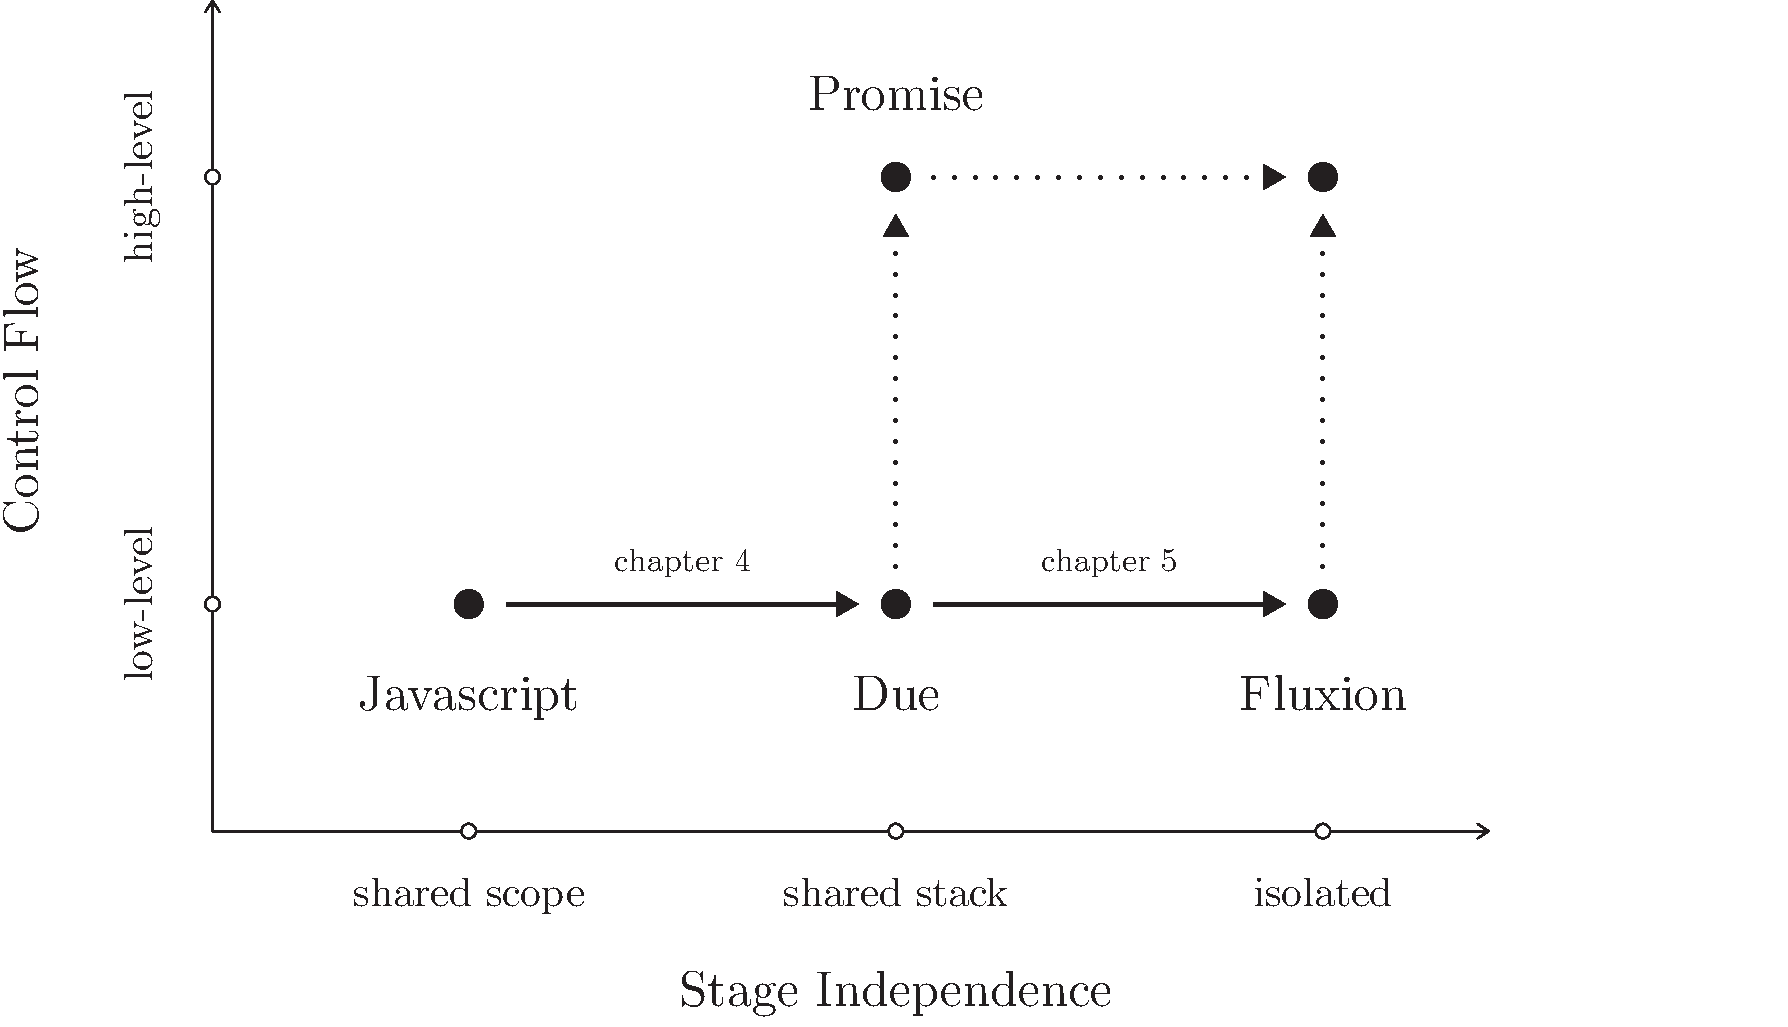
\includegraphics[width=1\textwidth]{../ressources/roadmap.pdf}
\caption{Roadmap}
\label{fig:chapter3:objectives:roadmap}
\end{figure}

\subsubsection{Rupture Point}

The execution of the pipeline architecture is well delimited in isolated stages.
Each stage has its own thread of execution, and is independent from the others.
On the contrary, the code of the event-loop is linear because of the continuation passing style and the common memory store.
% The message passing linking the callbacks is transparently handled by the event-loop.
However, the execution of the different callbacks are as distinct as the execution of the different stages of a pipeline.
The call stacks of two callbacks are distinct.
Therefore, an asynchronous function call represents the rupture between two call stacks.
It is a rupture point, and is equivalent to a data stream between two stages in the pipeline architecture.

Both the pipeline architecture and the event-loop present these rupture points.
The detection of rupture points allows to map a pipeline architecture onto the implementation following the event-loop model.
To allow the transformation from one to the other, this thesis studies the possibility to detect rupture points, and to distribute the global memory into the parts defined by these rupture points.
The detection of rupture points is addressed in chapter \ref{chapter4}.

It presents the extraction of a pipeline of operations from a Javascript application.
Indeed, such pipeline is similar to the one exposed by Promises.
The chapter proposes a simpler alternative to the latter called Dues.
However, these operations still require a global memory for coordination so they are not executed in parallel.

\subsubsection{Invariance}

% This transformation is important on two points.
% The conservation of the invariance.
% The equivalence between the coordinations.

The transformation should preserve the invariance as expressed by the developer to assure the correctness of the execution.
The partial ordering of events in a system, by opposition to total ordering, is sufficient to assure this correctness.
% This result was used by Lamport to prove the correctness of distributed systems.
The global memory is a way to assure the total ordering of events, and the message passing coordination is a way to assure partial ordering of events.
Therefore, to assure the correctness of the execution of a system, the state coordination with a global memory is equivalent to message passing coordination.
And it is possible, at least for some rupture points, to transform the global memory coordination into message passing while conserving the correctness of execution.

In order to preserve the invariance assured by the event-loop model after the transformation, each stage of the pipeline needs to have an exclusive access to memory.
The global memory needs not to be split into parts and distributed into each of the stages.
To assure the missing coordinations assured by the shared memory between the stages, the transformation should provide equivalent coordination with message passing.
The isolation and replacement of the global memory is fully address in chapter \ref{chapter5}, with the introduction of isolated containers called Fluxions.




% The invariance holds for the whole memory during the execution of each callback.
% As I explained in the previous section, this invariance is required to allow the concurrent execution of the different tasks.
% On the other hand, the invariance is explicit in the pipeline architecture, as all the stages have isolated memories.
% The coordination between these isolated process is made explicit by the developer through message passing.

% I argue that the state coordination between the callbacks requireing a global memory could be replaced by the message passing coordination used manually in the pipeline architecture.
% I argue that not all applications need concurrent access on the state, and therefore, need a shared memory.
% % Specifically, I argue that each state region remains roughly local to a stage during its modification.
% \nt{TODO review that, I don't know how to formulate these paragraphs. Identify the state and the data in the global memory.}

% \subsubsection{Transformation}

% This equivalence should allow the transformation of an event loop into several parallel processes communicating by messages.
% In this thesis, I study the static transformation of a program, but the equivalence should also hold for a dynamic transformation.
% I present the analyzis tools I developed to identify the state and the data from the global memory.
